\begin{figure*}
\centering
\begin{subfigure}[h]{0.45\textwidth}
\caption{}
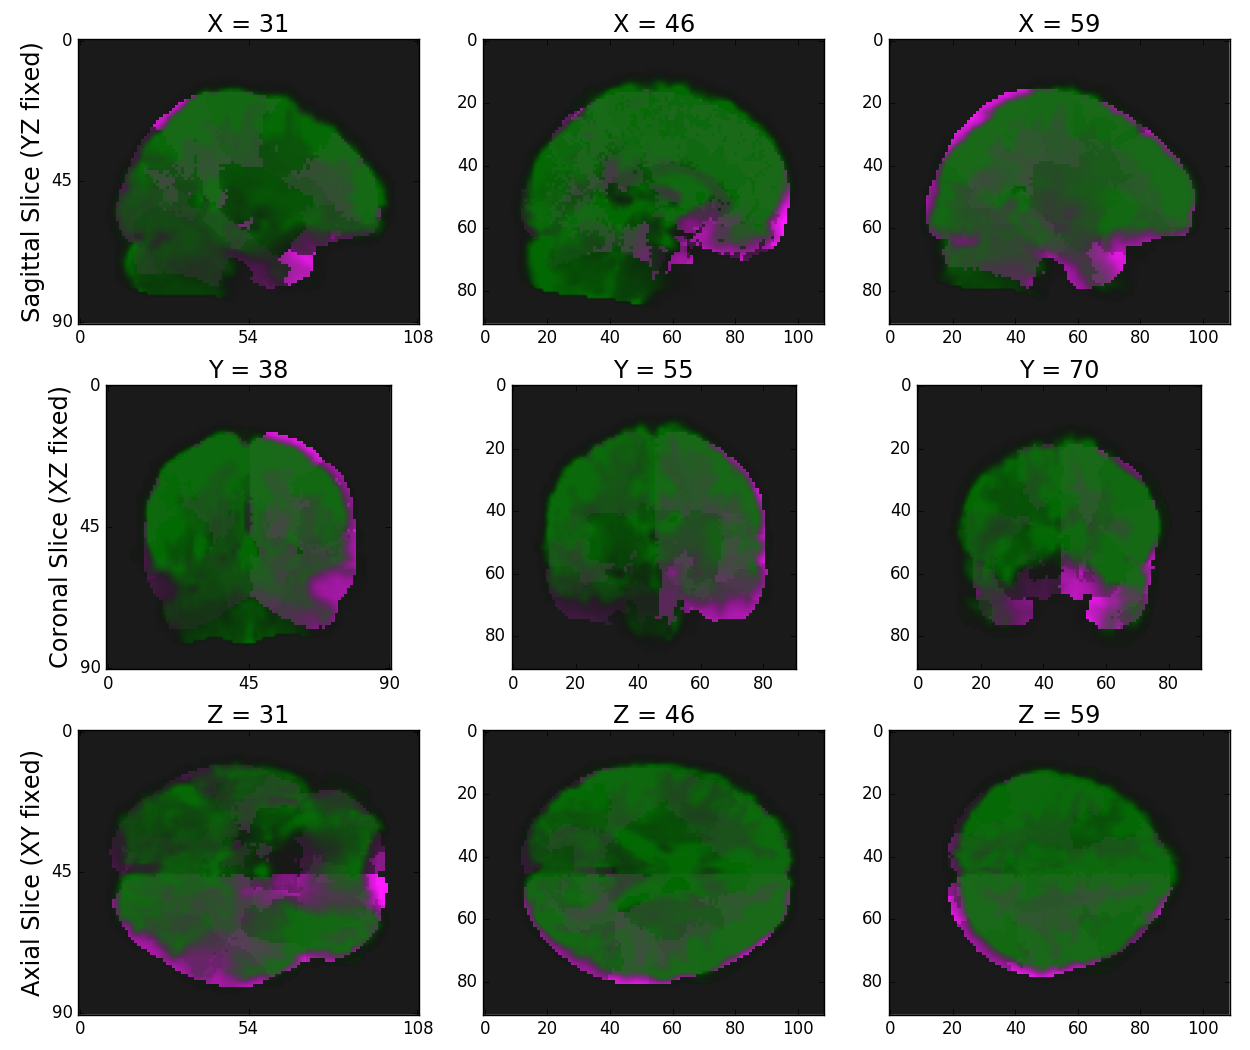
\includegraphics[width=\textwidth]{./qa_figs/fig_fmri_graph_overlap.png}
\label{fig:ov}
\end{subfigure}
\begin{subfigure}[h]{0.45\textwidth}
\caption{}
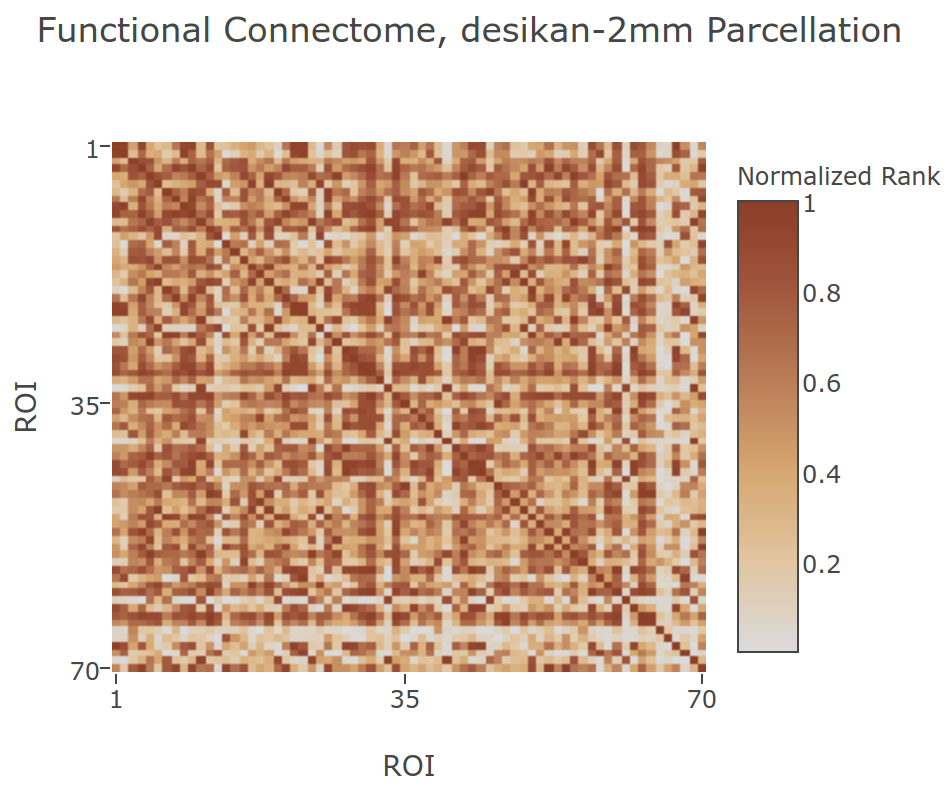
\includegraphics[width=\textwidth]{./qa_figs/fig_fmri_corr.png}
\label{fig:corr}
\end{subfigure}
\begin{subfigure}[h]{0.9\textwidth}
\caption{}
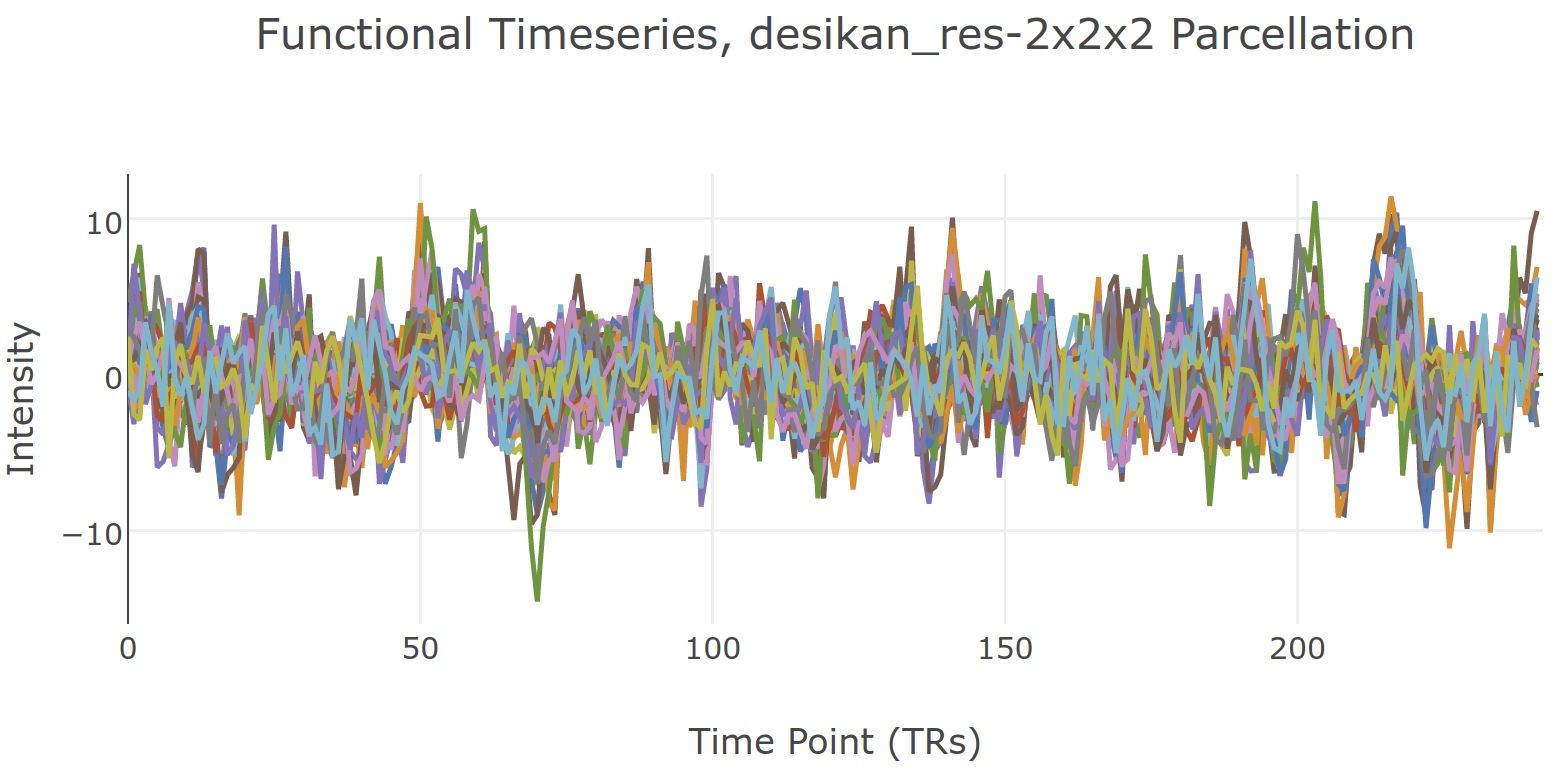
\includegraphics[width=\textwidth]{./qa_figs/fig_fmri_timeseries.png}
\label{fig:ts}
\end{subfigure}
\caption{\textbf{\ndmgf~Graph Generation QA}. For each parcellation, we visualize
(a)  the T1w image (green) over the parcellation (purple), the cleaned fMRI over the parcellation,
(b) the correlation matrix produced for each parcellated timeseries, and 
(c) the parcellated timeseries.}
\label{fig:fmri_graph}
\end{figure*}